\chapter{\'Etat de l'art sur la d\'etection de patrons de conception}



%L'approche SOMAD repose sur deux champs de recherches distincts: la d\'etection d'anti-patrons et l'extraction de connaissances depuis les traces d'association. La section \ref{rel1} pr\'esente les travaux de l'\'etat de l'art concernant la d\'etection de patrons et d'anti-patrons qu'ils soient orient\'es objets ou services. La section \ref{rel2}, quant \`a elle, pr\'esente les travaux de l'\'etat de l'art en acquisition de connaissances depuis les traces d'ex\'ecution. Finalement, la section \ref{soda} pr\'esente SODA, la seule approche existante pour la d\'etection d'anti-patrons SOA que nous avons propos\'ee dans \citep{Moha, Nayrolles, palma} et sur laquelle SOMAD est bas\'e.

%

%\section{D\'etection de Patrons et Anti-Patrons\label{rel1}}

%

%\comment{Voir journal paper + francis proposal + "Mining Rare Association Rules in the Datasets with Widely Varying Items? Frequencies" +  Cornelissen et al to get an overview of knowledge extraction from execution traces.}


Conserver une bonne qualit\'e architecturale est essentiel pour construire des syst\`emes maintenables et \'evolutifs. Les patrons et anti-patrons ont \'et\'e reconnus comme une des meilleures fa�ons d'exprimer ces pr\'eoccupations architecturales. Cependant, au contraire des anti-patrons orient\'es objet, la d\'etection de leurs \'equivalents orient\'es services en est encore \`a ses d\'ebuts.


Dans ce chapitre d\'edi\'e \`a l'\'etat de l'art sur la d\'etection de patrons de conception, nous verrons tout d'abord la d\'etection des anti-patrons objet suivi par la d\'etection de patrons SOA. Ensuite, une troisi\`eme sous section couvrira l'\'etat de l'art de la d\'etection d'anti-patrons SOA. Finalement, nous expliquerons le fonctionnement du seul outil, nomm\'e SODA, permettant la d\'etection automatique d'anti-patrons SOA.



\section{D\'etection d'anti-patrons orient\'es objets}


%\red{En total contraste avec la d\'etection d'anti-patrons SOA, la d\'etection d'anti-patrons objet est sujette \`a des recherches intensives depuis de nombreuses ann\'ees.

Ce champs de recherche est toujours largement ouvert, m\^eme si les contributions r\'ecentes se r\'ev\`elent plus incr\'ementales que r\'eelement nouvelles.

Un nombre important d'approches et d'outils existent pour la d\'etection d'anti-patrons objet \citep{Lanza2006, Moha2010, Kessentini2010,Kessentini2011} et de nombreux livres ont aussi port\'e sur le sujet.
En effet, \citet{Brown1998} ont produit un catalogue de 40 anti-patrons tandis que Beck, dans le livre \`a succ\`es \textit{Refactoring} de \citet{Fowler1999}, a identifi\'e 22 mauvaises odeurs de code (ou \textit{code smells} en anglais) qui doivent \^etre traqu\'ees et \'elimin\'ees afin d'avoir un code de meilleure qualit\'e.
\red{Un exemple simple d'anti-patron orient\'e objet est le \textit{``blob''}, aussi connu sous le nom de \textit{``god object''} (figure \ref{blob}), correspond \`a un contr�leur de grande taille (grand nombre d'attributs et de m\'ethodes) qui d\'epend de donn\'ees stock\'ees dans des classes adjacantes.

Le blob est une tr\`es grande classe qui d\'eclare de nombreux champs et m\'ethodes avec une faible coh\'esion.
Une classe de type contr�leur monopolise la majorit\'e du traitement effectu\'e par le syst\`eme, prend la majorit\'e des d\'ecisions et dirige le traitement eff\'ectu\'e par les autres classes.
De plus, il est fortement coupl\'e aux classes de donn\'ees adjacentes.}


\begin{figure}

\begin{center}

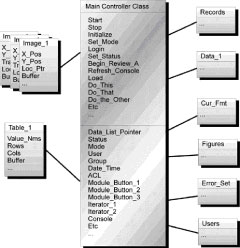
\includegraphics{media/blob.jpg}

\caption{Le blob objet\label{blob}}

\end{center}

\end{figure}


\red{Afin de d\'etecter un blob dans un programme \`a base d'objets, il faut identifier le nombre de classes de donn\'ees qui entourent un controleur, calculer sa coh\'esion, le nombre de champs et de m\'ethodes d\'eclar\'es.

}


Au sein des travaux sur les anti-patrons objet, certains sont particuli\`erement int\'eressants pour nos objectifs.
Notamment DECOR \citep{Moha2010} qui est une approche bas\'ee sur des r\`egles visant la sp\'ecification et la d\'etection de motifs dans le code ou la conception des syst\`emes objets.
Les motifs sont des morceaux de code ou de conception qui sont reconnaissables, car ils ont \'et\'e identifi\'es et nomm\'es dans le but de faciliter la communication entre les membres d'une m\^eme \'equipe et d'am\'eliorer la qualit\'e logiciel en g\'en\'eral.
Les auteurs de cette \'etude utilisent un langage sp\'ecifique au domaine (ou DSL) pour sp\'ecifier les motifs et, ensuite, ils g\'en\`erent automatiquement des algorithmes de d\'etection qui sont directement ex\'ecutables.
DECOR peut d\'etecter les anti-patrons objets avec une pr\'ecision de 60.5\% et un rappel de 100\%.
Une autre approche propos\'ee par \citet{Kessentini2011} a obtenues de meilleurs r\'esultats que DECOR et a apport\'e une construction automatique des r\`egles de d\'etection.
De plus, les auteurs ont utilis\'e des algorithmes g\'en\'etiques pour maximiser la d\'et\'ection via l'optimisation des ensembles de r\`egles.
Les algorithmes g\'en\'etiques imitent le processus de la s\'election naturelle pour produire des solutions approchant le r\'esultat optimal en un temps raisonnable.
Finalement, \citet{Khomh2011} ont \`a nouveau obtenu de meilleurs r\'esultats en utilisant des r\'eseaux bay\'esiens.
Les r\'eseaux bay\'esiens sont un mod\`ele probabiliste qui repr\'esentent des variables al\'eatoires et leurs d\'ependances conditionnelles gr�ce \`a un graphe dirig\'e acyclique (DAG).
Une alternative \`a la sp\'ecification par un langage d\'edi\'e, nomm\'ee SPARSE, a \'et\'e pr\'esent\'ee par \citet{Settas2011}.
SPARSE permet de d\'ecrire les anti-patrons en utilisant des ontologies OWL agr\'ement\'ees avec des r\`egles SWRL (\textit{Semantic Web Rule Language}) tandis que leurs occurrences sont test\'ees en utilisant le raisonneur s\'emantique Pellet \citep{Sirin2007}.
Un raisonneur s\'emantique est capable de d\'eduire des cons\'equences logiques depuis un ensemble de faits av\'er\'es.



D'autres travaux pertinents se sont focalis\'es sur la d\'etection d'anti-patrons sp\'ecifiquement li\'es aux performances et aux ressources syst\`emes.
Par exemple, \citep{Wong2010}, utilisent un algorithme g\'en\'etique pour la d\'etection de d\'efauts dans les logiciels.
Dans un autre travail pertinent, \citet{Parsons2007} s'occupe de la d\'etection d'anti-patrons de performance.
Il utilise une approche bas\'ee sur des r\`egles statiques et dynamiques visant les applications \`a base de composants (plus particuli\`erement les applications Java EE\footnote{Java Enterprise Edition, ou Java EE (anciennement J2EE), est une sp\'ecification pour la technologie Java de Sun Microsystems (Oracle) plus particuli\`erement destin\'ee aux applications d'entreprise.
}).



De plus, il existe une grande vari\'et\'e d'outils d\'evelopp\'es par l'industrie et la communaut\'e acad\'emique qui visent la d\'etection automatique d'anti-patrons dans les syst\`emes objet; les plus connus \'etant:  FindBugs, iPlasma, JDeodorant, PMD  et SonarQube \citep{Rutar}.




\section{D\'etection de patrons SOA}


Le catalogue actuel de patrons SOA est relativement riche. En effet, il existe de nombreux livres \citep{Erl2009, Daigneau2011} portant sur ce sujet et plus encore \citep{Rotem-Gal-Oz2012}.
Ces ouvrages fournissent de bonnes pratiques \`a adopter pour concevoir des applications \`a base de services.
Par exemple, \citet{Rotem-Gal-Oz2012} introduisent 23 patrons SOA et quatre anti-patrons suivi de discussions sur les raisons de leurs apparitions et les solutions \& probl\`emes qu'ils peuvent apporter.
Erl, quant \`a lui, introduit plus de 80 patrons SOA s\'epar\'es en quatre cat\'egories: architecturaux, impl\'ementation, s\'ecurit\'e et gouvernance \citep{Erl2009}.
Malgr\'e ce catalogue de patrons relativement dense, peu de techniques ont \'et\'e propos\'ees pour la d\'etection de patrons dans un environnement SOA.

Deux contributions sont particuli\`erement pertinentes dans le domaine de la d\'etection de patrons SOA.
Tout d'abord \citet{Upadhyaya2012a} ont identifi\'e des patrons de composition de services, c'est \`a dire, des services qui sont utilis\'es ensemble de fa�on r\'ep\'et\'ee tout en \'etant structurellement et fonctionnellement similaires.

Ces travaux pourraient \'egalement \^etre adapt\'es pour la correction d'anti-patrons.
La seconde approche est nomm\'ee SODOP (\textit{Service Oriented Dection Of Patterns}) et a \'et\'e propos\'ee par \citet{Demange2013}.
Cette approche, bas\'ee sur l'approche SODA \citep{Moha, Nayrolles, Palma2013}, propose de d\'etecter cinq patrons nouvellement d\'efinis en utilisant des cartes de r\`egles.
Les cartes de r\`egles sont des ensembles de m\'etriques qui peuvent \^etre statiques ou dynamiques, comme le couplage ou la coh\'esion.
Par la suite, ils g\'en\`erent des algorithmes de d\'etection et les appliquent sur un syst\`eme \`a base de services instrumentalis\'e pour ex\'ecuter des sc\'enarios.
Une explication approfondie de SODA, l'approche sur laquelle SODOP est bas\'ee, sera fournie dans la section \ref{soda}.
 Outre ces deux contributions majeures, il existe quelques travaux sur la d\'etection de patrons SOA en utilisant la similarit\'e entre les services \citep{Liang2006}, ou les \textit{workflows} \citep{Weijters2003,Dijkman2009}.
Cependant, ces travaux sont diff\'erents, car ils ne cherchent pas \`a \'evaluer la qualit\'e globale d'un syst\`eme, au contraire de SODOP.
En effet, SODOP est la seule approche qui vise clairement \`a d\'eterminer la qualit\'e de conception de syst\`emes \`a base de services dans le but de faciliter la maintenance et l'\'evolution de tels syst\`emes.



\red{A titre d'exemple, le fa�ade (figure \ref{facade}) est un patron SOA permettant d'obtenir une abstraction sup\'erieure.
Ce patron est inspir\'e par des patrons similaires nomm\'es Remote Facade \citep{Fowler1999} et Decoupled Contract \citep{Erl2009}.
Une facade peut \^etre responsable de l'orchestration du syst\`eme ou \^etre utilis\'ee pour masquer des syst\`emes l\'egataires.
}


\begin{figure}

\begin{center}

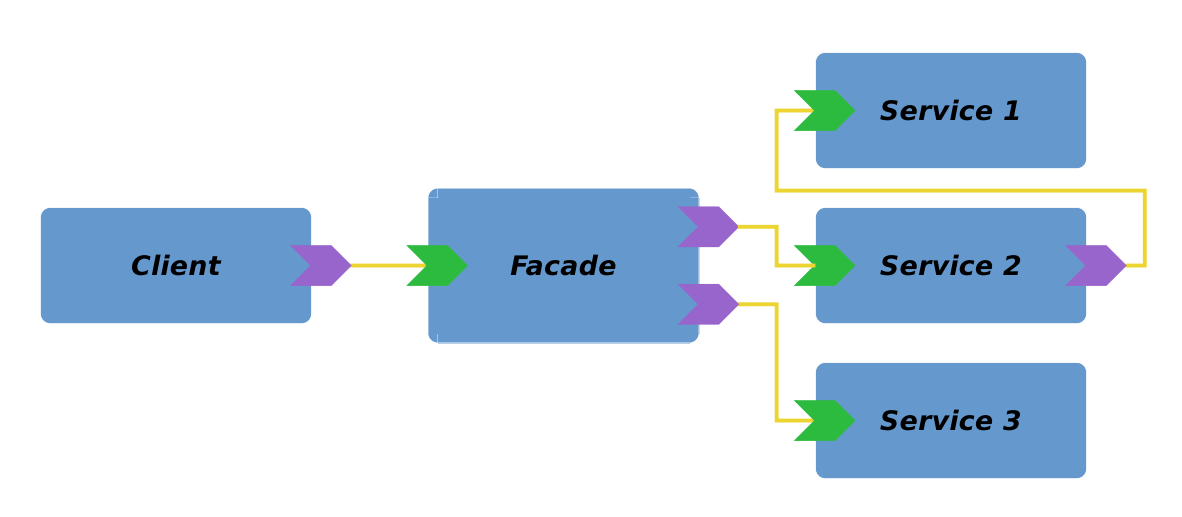
\includegraphics[scale=0.2]{media/facade.png}

\caption{Le patron facade \citep{Demange2013}\label{facade}.}

\end{center}

\end{figure}


\red{Pour d\'etecter un patron fa�ade, une des m\'ethodes consiste \`a calculer son temps de r\'eponse et son ratio de couplage entrant sur le couplage sortant.
Une fa�ade devrait avoir un fort temps de r\'eponse puisqu'elle offre un point d'entr\'ee au syst\`eme \`a de nombreux clients et un faible ratio couplage entrant / sortant puisqu'elle cache l'impl\'ementation de nombreux autres services \citep{Demange2013}.
}




\section{D\'etection d'anti-patrons SOA}


Contrairement aux patrons SOA, les anti-patrons ont beaucoup moins \'et\'e \'etudi\'es par la communaut\'e.
En effet, \red{la litt\'erature sur le sujet est plut\^ot r\'eduite}.
De ce fait, la plupart des r\'ef\'erences sont des pages Internet o� des d\'eveloppeurs SOA partagent leurs exp\'eriences sur les bonnes pratiques SOA  \citep{LubaCherbakovMamdouhIbrahim2005}.
Il existe tout de m\^eme quelques ouvrages cons\'equents, notamment \citep{Dudney2003} qui constitue le premier livre sur les anti-patrons SOA.
Cet ouvrage r\'epertorie 53 anti-patrons li\'es \`a l'architecture et l'impl\'ementation de syst\`emes JEE (\textit{Java 2 Platform Enterprise Edition}), tels que les EJB (\textit{Enterprise Java Beans}, JSP (\textit{JavaServer Pages}) ou encore les \textit{Servlets}.
Malgr\'e la pertinence de ce livre pour nos recherches, il ne propose aucune approche pour la d\'etection automatique de ces patrons.
\red{De plus, ces anti-patrons sont uniquement applicables aux syst\`emes JEE alors que la plupart d'entre eux ne sont que des variantes des \textit{Tiny Servic}e et \textit{Multi Service} \'evoqu\'es dans l'introduction.
} Kral et Zemkicka ont eux aussi apport\'e une contribution significative aux anti-patrons SOA.
En effet, ils ont sp\'ecifi\'e sept anti-patrons SOA directement li\'es \`a l'utilisation de pratiques objets.
Une fois encore, la question de la d\'etection automatique de ces anti-patrons n'est pas \'evoqu\'ee \citep{Kral2009}.


Bien que le catalogue global d'anti-patrons SOA commence \`a gagner un certain int\'er\^et et grossit de jour en jour, seulement de quelques contributions existent pour la d\'etection automatique d'anti-patrons dans des environnements SOA.
En effet, seulement deux contributions sont \`a signaler \citep{Eck2009} en plus de la n�tre --- SODA --- d\'ecrite dans trois publications diff\'erentes \citep{Moha, Nayrolles, Palma}.
D'autres auteurs proposent une technique pour d\'ecouvrir des anti-patrons d\'ependant des flux de donn\'ees, comme par exemple, des donn\'ees manquantes, inconsistantes ou encore supprim\'ees trop t�t.
Ils d\'etectent ces anti-patrons sp\'ecifiques en analysant les d\'ependances entre les donn\'ees dans les flux d'ex\'ecution et les probl\`emes qui pourraient appara�tre en cas de manipulation non optimale \citep{Eck2009}.
Cette \'etude, bien que pertinente pour nos recherches, se concentre sur les anti-patrons SOA li\'es aux flux de donn\'ees alors que nous cherchons \`a d\'etecter les anti-patrons SOA distribu\'es dans tout le syst\`eme et non reli\'e \`a une activit\'e particuli\`ere.




\section{SODA, l'approche de l'\'etat de l'art pour la d\'etection automatique d'anti-patrons SOA\label{soda}.}


Comme mentionn\'e plus haut, l'unique approche automatique disponible pour la d\'etection d'anti-patrons SOA est SODA \citep{Moha, Nayrolles, Palma}.
SODA repose sur un langage de r\`egles qui permet la sp\'ecification d'anti-patrons en utilisant un ensemble de m\'etriques.
Un processus g\'en\'erique transforme les sp\'ecifications en algorithmes de d\'etection \`a ex\'ecuter sur les syst\`emes \`a analyser.
SODA est compos\'e des trois \'etapes d\'ecrite ci-apr\'es et illustr\'ees  par la figure \ref{fig:The-SODA-approach}:


\begin{figure*}


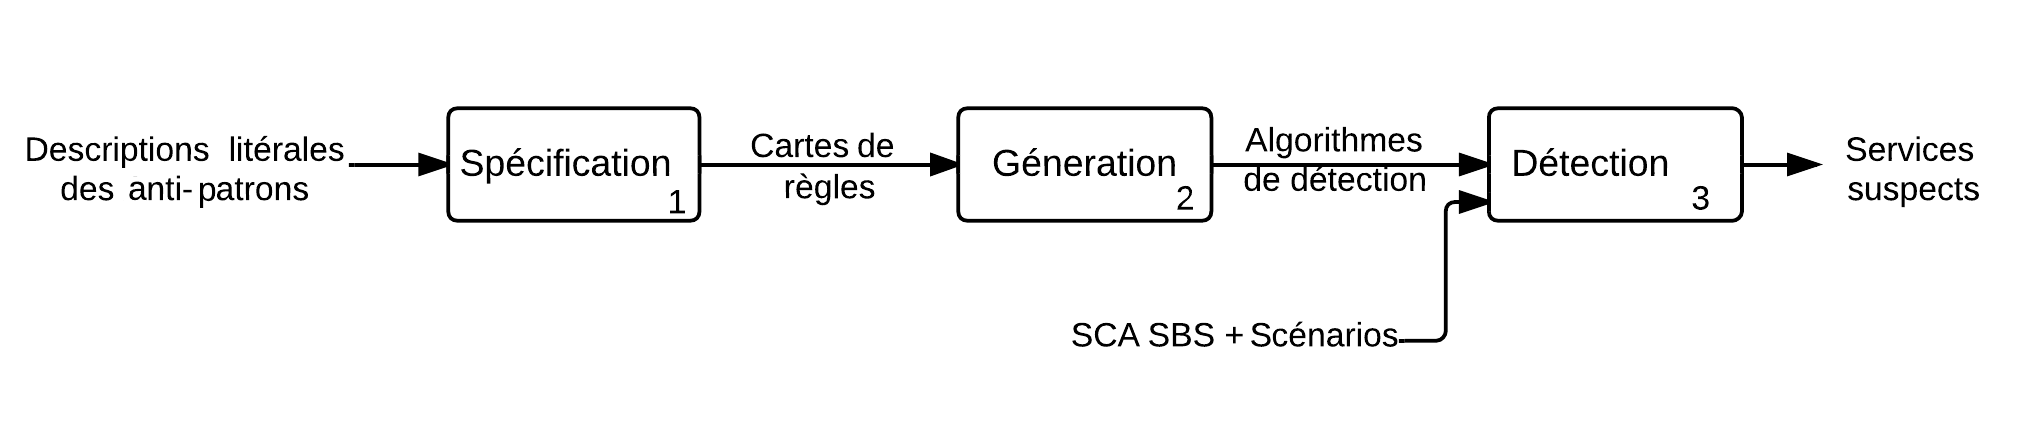
\includegraphics[scale=0.21]{media/SODA.png}%


\caption{\label{fig:The-SODA-approach}L'approche SODA}

\end{figure*}



\textit{Sp\'ecification d'anti-patrons SOA:} Cette \'etape identifie les propri\'et\'es relevant de la sp\'ecification des anti-patrons SOA.
Ces descriptions textuelles sont pr\'esent\'ees dans le tableau \ref{tab:List-of-SOA}.
Les propri\'et\'es correspondent de mani\`ere g\'en\'erale \`a des m\'etriques, par exemple, la coh\'esion, le couplage, le nombre de m\'ethodes, le temps de r\'eponse et la disponibilit\'e.
De plus, ces propri\'et\'es sont utilis\'ees comme base d'un DSL, qui prend la forme d'un langage \`a base de r\`egles pour la sp\'ecification d'anti-patrons SOA.
La sp\'ecification finale est une \textit{carte de r\`egles}, qui est une composition de r\`egles combinant des m\'etriques.



\begin{longtable}{p{.95\textwidth}}

\tabularnewline

\hline 

\textbf{Multi-Service}, aussi connu sous le nom  ``God object'' dans le paradigme objets,
correspond \`a un service qui impl\'emente une \textbf{multitude de m\'ethodes} faisant r\'ef\'erence \`a diff\'erentes abstractions m\'etiers et techniques.
Il agr\`ege beaucoup d'abstractions diff\'erentes \`a l'int\'erieur d'un un m\^eme service.
Un tel service est difficilement r\'eutilisable \`a cause de la \textbf{faible coh\'esion} entre ses m\'ethodes et il est souvent non disponible aux utilisateurs finaux \`a cause de sa charge, laquelle peut introduire de fort temps de r\'eponse \citep{Dudney2003}.


\begin{center}

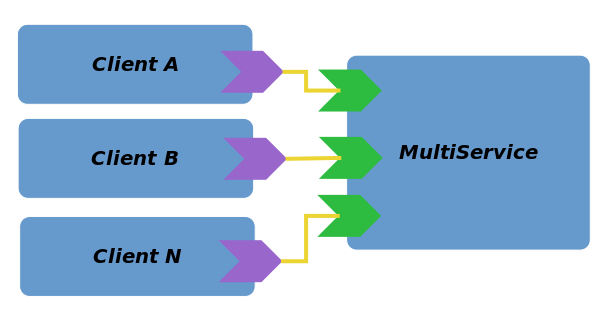
\includegraphics[scale=0.3]{media/multisca.png}

\end{center}

\vspace{-0.5cm}

\tabularnewline

Le \textbf{Tiny Service} est un petit service avec \textbf{peu de m\'ethodes} qui impl\'ementent uniquement une partie d'une abstraction.
Un tel service requiert plusieurs services coupl\'es pour \^etre utilis\'e correctement.
De ce fait, le Tiny Service introduit une complexit\'e importante dans le d\'eveloppement.
Dans certains cas extr\^eme, le Tiny Service est limit\'e \`a \textbf{une m\'ethode unique}, avec pour cons\'equence de nombreux services impl\'ementant l'ensemble des fonctionnalit\'es sous-jacentes \citep{Dudney2003}.


\begin{center}

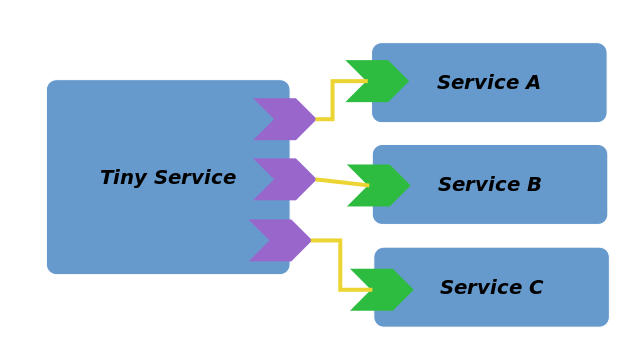
\includegraphics[scale=0.3]{media/Tinysca.png}

\end{center}

\vspace{-0.5cm}

\tabularnewline

Le \textbf{Chatty Service} correspond \`a un service qui \textbf{\'echange beaucoup de donn\'ees} de type primitif.
Le Chatty Service est aussi caract\'eris\'e par un \textbf{grand nombre d'invocations}; il \textit{discute} \'enorm\'ement avec le reste du syst\`eme \citep{Dudney2003}.


\begin{center}

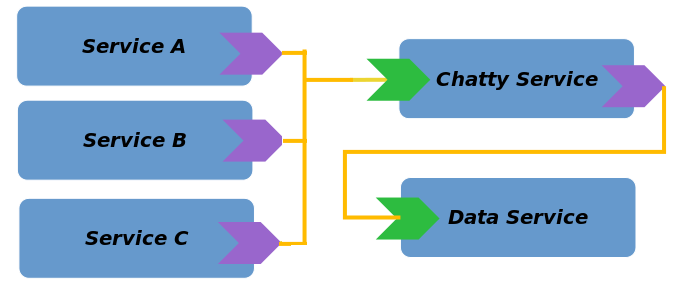
\includegraphics[scale=0.3]{media/chattysca.png}

\end{center}

\vspace{-0.5cm}

\tabularnewline

Le \textbf{Knot} est un ensemble de services \textbf{tr\`es peu coh\'esifs} et \textbf{fortement coupl\'es entre eux}.
Ces services sont de ce fait, tr\`es difficilement r\'eutilisables.
\`A cause de la complexit\'e induite de l'architecture, la disponibilit\'e de ces services peut \^etre faible et leur temps de r\'eponse \'elev\'e \citep{Rotem-Gal-Oz2012}.


\begin{center}

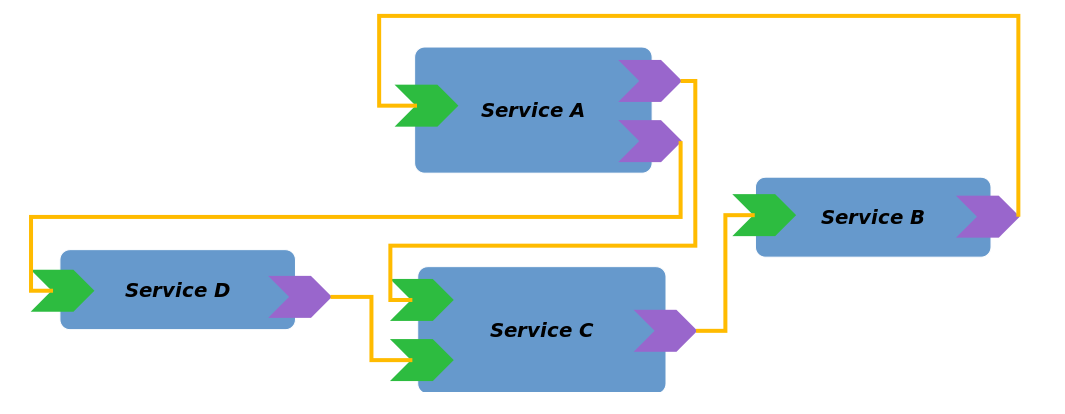
\includegraphics[scale=0.3]{media/knotsca.png}

\end{center}

\vspace{-0.5cm}

\tabularnewline

Le \textbf{Bottleneck Service} est un service \textbf{tr\`es utilis\'e} par le reste du syst\`eme (les autres services ou clients).
Il a un \textbf{fort couplage entrant et sortant}.
Son temps de r\'eponse peut \^etre \'elev\'e car il est utilis\'e par de nombreux clients, et les clients doivent attendre la r\'eponse des couches inf\'erieures.
De plus, sa disponibilit\'e peut \^etre faible \`a cause du trafic engendr\'e.


\begin{center}

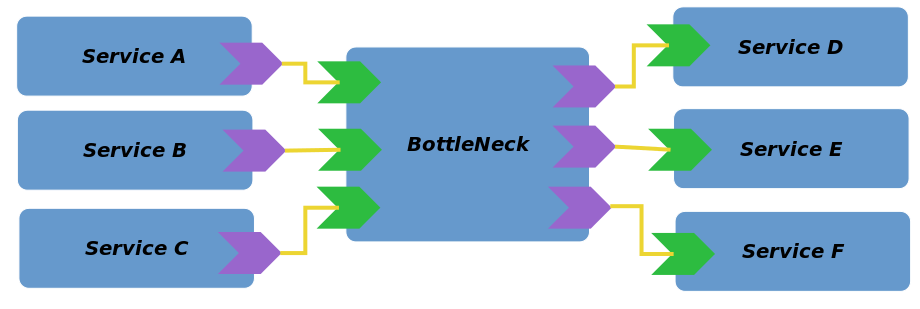
\includegraphics[scale=0.3]{media/bottlesca.png}

\end{center}

\vspace{-0.5cm}

Le \textbf{Service Chain}, aussi connu sous le nom de ``Message Chain'' dans les syst\`emes objets, correspond \`a \textbf{une cha�ne de services}.
Le Service Chain appara�t quand la requ\^ete d'un client est compl\'et\'ee par une invocation cons\'ecutive et successive de services.
Ce genre de \textbf{cha�nes de d\'ependances} engendrent des \textbf{invocations transitives}.


\begin{center}

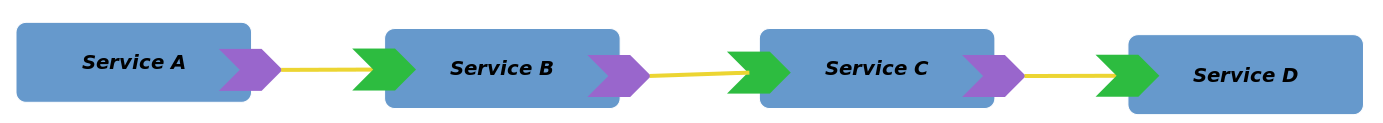
\includegraphics[scale=0.28]{media/chainsca.png}

\end{center}

\vspace{-0.5cm}

\tabularnewline

\hline 

\caption{Anti-patrons SOA \citep{Moha} \label{tab:List-of-SOA}.}

\end{longtable}


\textit{G\'en\'eration des algorithmes de d\'etection:} Le but de cette \'etape est de g\'en\'erer automatiquement des algorithmes de d\'etection en visitant les cartes de r\`egles sp\'ecifi\'ees \`a l'\'etape pr\'ec\'edente.
Ce processus est automatique et g\'en\`ere des algorithmes de d\'etection directement ex\'ecutables.



\textit{D\'etection des anti-patrons SOA:} Cette troisi\`eme et derni\`ere \'etape consiste \`a appliquer les algorithmes g\'en\'er\'es sur un syst\`eme \`a base de services.
Cette \'etape permet la d\'etection automatique des anti-patrons SOA en utilisant un ensemble de sc\'enarios pr\'ed\'efinis qui invoquent les interfaces des services.
\`A la fin de cette \'etape, les services du syst\`eme suspect\'es d'\^etre impliqu\'es dans un anti-patron SOA sont identifi\'es.



Bien qu'efficace et pr\'ecis, SODA est une approche intrusive, car elle requiert un ensemble de sc\'enarios qui invoquent concr\`etement les interfaces des services du syst\`eme.
De plus, son analyse dynamique implique des propri\'et\'es propres aux syst\`emes SCA (\textit{Service Component Architecture}, une sourcouche au SOA).
En effet, l'analyse dynamique de SODA repose sur le tissage d'aspects qui est une fonctionnalit\'e de la programmation orient\'ee aspects qui consiste \`a ins\'erer du code, qui s'ex\'ecutera avant ou apr\`es une m\'ethode donn\'ee,  dans le code m\'etier de l'application vis\'ee.
SCA est la seule technologie SOA \`a supporter cette fonctionnalit\'e.



\section{Conclusion}


De nombreux travaux ont \'et\'e men\'es pour la d\'etection d'anti-patrons dans les syst\`emes orient\'es objets, notamment les approches d\'erivant ou am\'eliorant celle de \citep{Moha2010}.
Pour le monde des applications \`a base de services, la communaut\'e a cr\'e\'e un catalogue tr\`es dense de patrons SOA, mais une seule approche vise leur d\'etection dans le but de d\'eterminer la qualit\'e globale du syst\`eme pour faciliter la maintenance et l'\'evolution de tels syst\`emes.
Cette approche pr\'esent\'ee par \textit{Demange et al.} a \'et\'e inspir\'ee par une autre approche nomm\'ee SODA -- que nous avons propos\'ee en 2012 \citep{Moha, Nayrolles, Palma}.
SODA se concentre, elle aussi, sur la facilitation de la maintenance et de l'\'evolution des applications \`a base de services, mais en d\'etectant les anti-patrons SOA.
Malgr\'e que ces deux approches soient pertinentes et efficaces, elle sont limit\'ees par plusieurs points:


\begin{itemize}

\item Elles n\'ecessitent d'avoir un bon niveau de contr�le sur le syst\`eme analys\'e;
en particulier elles doivent avoir acc\`es aux interfaces des services du syst\`eme;

\item Elles n\'ecessitent de poss\'eder des sc\'enarios pertinents;

\item SODA est majoritairement bas\'e sur des m\'etriques statiques alors que
SODOP utilise une part plus importante de m\'etriques dynamiques;

\item Techno-centrique (SCA) puisque bas\'e sur le tissage d'aspects.


\end{itemize}


Notre objectif est de reprendre les forces de ces approches comme la sp\'ecification d\'eclarative des anti-patrons via un language d\'edi\'e et la g\'en\'eration automatique d'algorithmes de d\'etection.
N\'eanmoins, nous voulons nous abstraire de la technologie du syst\`eme analys\'e, en nous appuyant sur des donn\'ees qui refl\`etent la nature hautement dynamique des SBSs.
Nous souhaitons aussi \'eviter toute intrusion dans le fil d'ex\'ecution normal du syst\`eme vis\'e.

